\setcounter{chapter}{1}
\chapter{Optical waveguides}
\section{Geometrical-optics description}
\subsection{Step-index (SI) waveguides}
	\begin{wrapfigure}[7]{l}{6cm}
	\vspace{-5mm}
	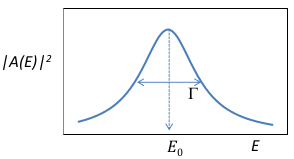
\includegraphics[scale=0.4]{ch1/image1.png}
	\captionof{figure}{ }
	\end{wrapfigure}
Dans un premier temps, on va seulement considérer la cas à deux dimensions : 
la lumière se propage dans un plan ($xy$ pour les guides plans, $rz$ pour les cylindriques). 
Pour l'instant, considérons $b$ comme étant infini. Généralement, le cœur mesure 9-10 microns
alors que la gaine est de 125 microns (vient ensuite le coating pour éviter les microcourbures).\\

	\begin{wrapfigure}[11]{r}{7cm}
	\vspace{-9mm}
	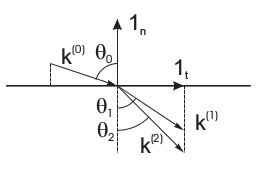
\includegraphics[scale=0.6]{ch1/image2.png}
	\captionof{figure}{ }
	\end{wrapfigure}
Effectuons une coupe dans le plan $rz$ de la fibre. En optique géométrique, il faut que la dimension physique dans laquelle la lumière se propage soit plus grand que la longueur d'onde. Autrement dit
\begin{equation}
\lambda \ll a,b
\end{equation}
Ceci est nécessaire afin de pouvoir modéliser la propagation par des rayons. Nous faisons l'hypothèse
que le cœur et la gaine sont des diélectriques homogènes\footnote{Utiliser un conducteur n'a pas de sens
: mouvement des charges libres, effets joule, \dots} où l'on suppose $n_1>n_2$, les indices de
réfractions du cœur et de la gaine. Nous verrons plus tard qu'il s'agit en fait d'une condition
nécessaire. Nous ferons aussi l'hypothèse d'un milieu sans pertes et invariant pour une translation
selon $z$ (pas de courbures).\\

La loi de Snell-Descartes exprime le changement de direction d'un faisceau lors de la traversée
d'une paroi. Chaque milieu à une capacité à "ralentir" la lumière, caractérisé par son indice
de réfraction $n\equiv c/v$
\begin{equation}
n_1 \sin\theta_1=n_2 \sin\theta_2
\end{equation}
Si $n_1>n_2$, le faisceau réfracté se rapproche plus rapidement du dioptre : le rayon est élevé alors
que dans le cas contraire, il est "rabattu". Dans le premier cas, le rayon peut remonter jusqu'à
l'horizontale $(\pi/2)$. Au dessus de cet angle, il sera totalement réfléchi : c'est le phénomène
de réflexion totale\footnote{Pour l'histoire, ceci explique pourquoi un diamant ne brille pas dans
l'eau.}\\


	\begin{wrapfigure}[9]{r}{7.5cm}
	\vspace{-9mm}
	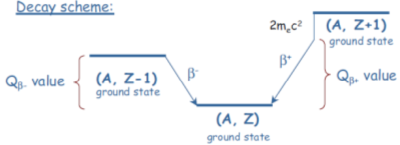
\includegraphics[scale=0.6]{ch1/image3.png}
	\captionof{figure}{ }
	\end{wrapfigure}
Considérons le rayon vert ci-contre. Initialement dans l'air, il rencontre l'interface air-verre ($
n_1$) ou il y a des réflexions. Ensuite, il rencontre l'interface cœur-gaine où on observe un 
phénomène de réflexion partielle et de réfraction. Il est possible d'avoir une \textbf{réflexion
totale} si le rayon a une incidence assez rasante et si $n_1>n_2$.\\

Regardons le cas particulier d'un angle critique (rouge). En appliquant la loi de S-D, on trouve
\begin{equation}
\left.\begin{array}{ll}
{n_0}\sin {\theta _i} &= {n_1}\sin {\theta _r}\\
{n_0}\sin {\theta _{ic}} &= \sin {\theta _{ic}} = {n_1}\sin {\theta _{rc}} = {n_1}\cos {\Phi _c}\\
{n_1}\sin {\Phi _c} &= {n_2}\sin \frac{\pi }{2} = {n_2}
\end{array}\right\}\cos {\Phi _c} = \sqrt {1 - {{\sin }^2}{\Phi _c}} = \sqrt {1 - {{\left( {{{{n_2}} \mathord{\left/
 {\vphantom {{{n_2}} {{n_1}}}} \right.
 \kern-\nulldelimiterspace} {{n_1}}}} \right)}^2}}
\end{equation}
où la première ligne correspond à l'interface air-cœur et la dernière au cas de réflexion totale. On 
peut ainsi trouver une expression pour l'angle critique. \\

\cadre{Le rayon sera guidé si\begin{equation}
\Phi  > {\Phi _c}
\end{equation}}\ \\

\begin{wrapfigure}[6]{l}{7.5cm}
	\vspace{-5mm}
	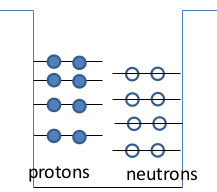
\includegraphics[scale=0.6]{ch1/image4.png}
	\captionof{figure}{ }
	\end{wrapfigure}
L'\textbf{ouverture numérique} renseigne le "cône d'acceptance" des rayons, afin que ceux-ci soient
guidés. Par définition
\begin{equation}
NA \buildrel \Delta \over = {n_0}\sin {\theta _{ic}} = {n_1}\sqrt {1 - {{\left( {{{{n_2}} \mathord{\left/
 {\vphantom {{{n_2}} {{n_1}}}} \right.
 \kern-\nulldelimiterspace} {{n_1}}}} \right)}^2}}  = \sqrt {{n_1}^2 - {n_2}^2} 
\end{equation}
Souvent on retrouve cette information dans les data-sheet pas pas $n_1$ et $n_2$, car l'AN est plus
facile à mesurer. On utilise souvent l'\textbf{indice de réfraction normalisé} $\Delta n \buildrel \Delta \over = {{\left( {{n_1} - {n_2}} \right)} \mathord{\left/
 {\vphantom {{\left( {{n_1} - {n_2}} \right)} {{n_1}}}} \right.
 \kern-\nulldelimiterspace} {{n_1}}}$ ainsi que l'indice de réfraction moyen $\bar n \buildrel \Delta \over = {{\left( {{n_1} + {n_2}} \right)} \mathord{\left/
 {\vphantom {{\left( {{n_1} + {n_2}} \right)} 2}} \right.
 \kern-\nulldelimiterspace} 2}$.\\
 
En pratique, on rencontre souvent un guidage dit faible : l'angle d'incidence est très proche de 
$90^\circ $ et on dit alors que $n_1\approx n_2$. Plus l'AN est grande, plus la propagation sera rapide. Un ordre de grandeur usuel pour celle-ci est de 0.2.

\subsubsection{Multipath dispersion (or Modal dispersion)}

\begin{wrapfigure}[8]{r}{4.5cm}
	\vspace{-5mm}
	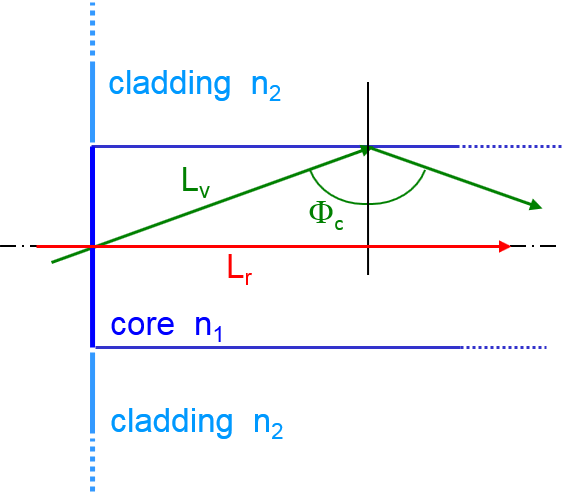
\includegraphics[scale=0.34]{ch1/image5.png}
	\captionof{figure}{ }
	\end{wrapfigure}
Le problème c'est qu'un rayon qui se propage sur l'axe ne va pas faire le même parcours que 
celui qui fait des zigzag. La vitesse de groupe est la même, mais il y aura un délai associé 
à cette différence de chemin entre les deux. Pour calculer ce délai, on s'intéresse à la différence
de chemin $\delta l$ entre les deux rayons (rouge et vert) à l'aide d'un joli triangle rectangle
\begin{equation}
\delta l = {L_v} - {L_r} = {L_r}\left( {{1 \mathord{\left/
 {\vphantom {1 {\sin {\Phi _c}}}} \right.
 \kern-\nulldelimiterspace} {\sin {\Phi _c}}}} \right) - {L_r} = {L_r}\left[ {\left( {{{{n_1}} \mathord{\left/
 {\vphantom {{{n_1}} {{n_2}}}} \right.
 \kern-\nulldelimiterspace} {{n_2}}}} \right) - 1} \right]
\end{equation}
Il faut ensuite sommer ceci sur la longueur $L$ de la fibre 
\begin{equation}
\Delta L = \sum {\delta l}  = L\left[ {\left( {{{{n_1}} \mathord{\left/
{\vphantom {{{n_1}} {{n_2}}}} \right.
\kern-\nulldelimiterspace} {{n_2}}}} \right) - 1} \right]
\end{equation}
En supposant que la vitesse de phase $(c/n)$ vaut à peu près la vitesse de groupe, on trouve
\begin{equation}
\Delta t = \frac{{\Delta L}}{{{c \mathord{\left/
 {\vphantom {c {{n_1}}}} \right.
 \kern-\nulldelimiterspace} {{n_1}}}}} = \frac{L}{c}{n_1}\left[ {{{\left( {{n_1} - {n_2}} \right)} \mathord{\left/
 {\vphantom {{\left( {{n_1} - {n_2}} \right)} {{n_2}}}} \right.
 \kern-\nulldelimiterspace} {{n_2}}}} \right] = \frac{L}{c}{n_1}\left[ {{{\left( {{n_1}\Delta n} \right)} \mathord{\left/
 {\vphantom {{\left( {{n_1}\Delta n} \right)} {{n_2}}}} \right.
 \kern-\nulldelimiterspace} {{n_2}}}} \right]
\end{equation}
où encore
\begin{equation}
\Delta t = \frac{L}{c}\Delta n\frac{{{n_1}^2}}{{{n_2}}}
\end{equation}
Une grande AN ($\propto \sqrt{\Delta n})$ facilité l'injection dans la lumière, mais un grand $\Delta t$ $(\propto\Delta n)$ limite le taux de bit.

\begin{center}
	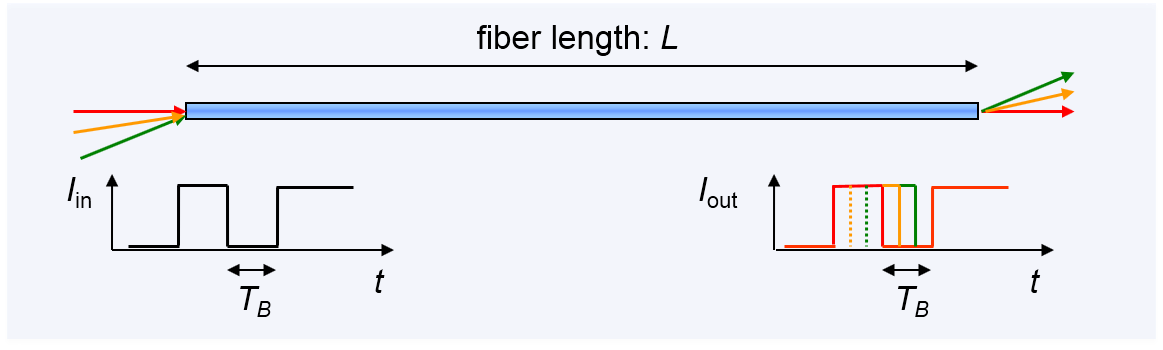
\includegraphics[scale=0.4]{ch1/image6.png}
	\captionof{figure}{ }
\end{center}

S'il y a une différence de vitesse de groupe, l'information va avoir tendance à s'étaler dans le 
temps. Les flancs vont alors s'étaler et il ne sera plus disponible de distinguer 0 et 1. Il faut que
cette dispersion temporelle soit inférieure au temps d'un bit : $\Delta t < T_B = 1/B$. Dès lors, 
$B\Delta t < 1 \Leftrightarrow B\frac{L}{c}{n_1}\left[ {{{\left( {{n_1}\Delta n} \right)} \mathord{\left/
 {\vphantom {{\left( {{n_1}\Delta n} \right)} {{n_2}}}} \right.
 \kern-\nulldelimiterspace} {{n_2}}}} \right] < 1$. On en tire (sous l'hypothèse que la taille du 
 cœur est grande par rapport à $\lambda$\\
 
 \cadre{\begin{equation}
 BL < \frac{c}{{\Delta n}}\frac{{{n_2}}}{{n_1^2}}
 \end{equation}}\ \\
 
Le produit $BL$ est donc bien un paramètre important pour une fibre. Celui-ci nous informe qu'un
signal de 200Mbits/s ne peut être transmis que sur une distance de 100m pour une fibre Si multimode. 

\newpage
\subsection{Graded-index (GI) fibers}
Pour réduire le délai entre les rayons guidés, on peut utiliser des fibres à \textbf{gradient} 
d'indice. L'indice change dans le cœur : élevé au centre (ralenti les rayons) et diminue ensuite 
(ralentis un peu moins les rayons)\footnote{Voir notes slides 10 et 11 pour plus de détails.}. 

\begin{center}
	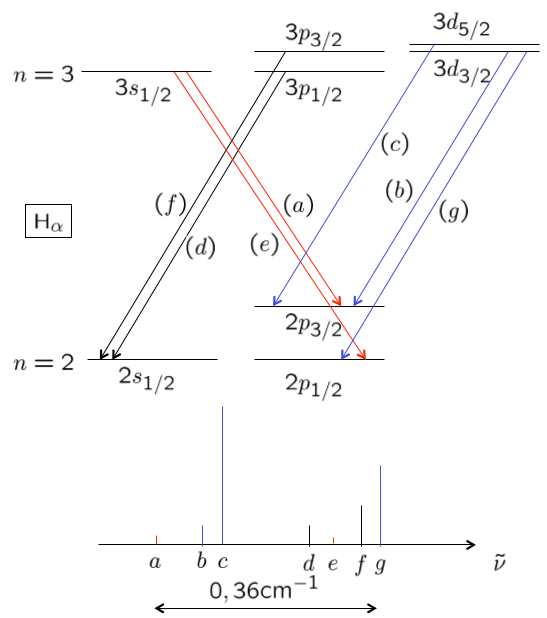
\includegraphics[scale=0.5]{ch1/image8.png}
	\captionof{figure}{ }
\end{center}

\begin{center}
	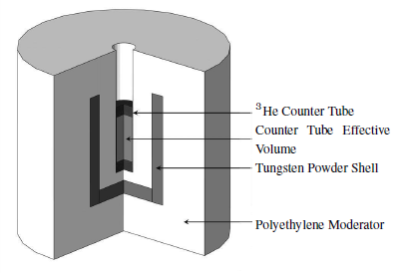
\includegraphics[scale=0.5]{ch1/image9.png}
	\captionof{figure}{ }
\end{center}


\subsubsection{Limitations of the simple two-dimensional geometrical optics description:}

\begin{wrapfigure}[5]{r}{8cm}
	\vspace{-5mm}
	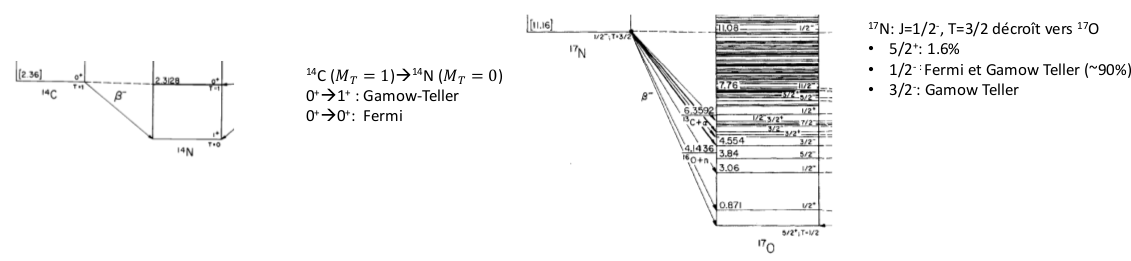
\includegraphics[scale=0.45]{ch1/image7.png}
	\captionof{figure}{ }
	\end{wrapfigure}
Jusqu'ici nous avons considérer que les rayons se situent uniquement dans des plans $xz/rz$. Or, 
certains rayons peuvent être obliques, hélicoïdaux, \dots\ De plus, que se passe-t-il si le 
cœur a une dimension proche de la longueur d'onde ? Il faut une approche EM!

\section{Electromagnetic analysis – Fields and modes}
\subsection{Step-index planar waveguides}

\begin{wrapfigure}[8]{r}{7cm}
	\vspace{-5mm}
	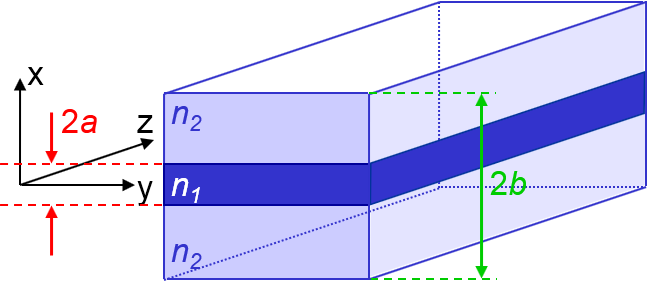
\includegraphics[scale=0.4]{ch1/image10.png}
	\captionof{figure}{ }
	\end{wrapfigure}
Nous allons commencer par le cas d'un guide d'onde plan. L'idée est de résoudre les équations de 
Maxwell afin de trouver une solution qui satisfait aux conditions limites, continuité, \dots\ soit 
un problème aux valeurs propres d'un certain opérateur différentiel (le propagateur) agissant sur un 
champ.\\

Nous allons faire plusieurs hypothèses
\begin{enumerate}
\item Matériau simple : diélectrique, non magnétique, linéaire, isotropique et sans perte. En gros,
juste $n_1$ et $n_2$ à prendre en compte.
\item Homogène : toujours $n_1$ dans le cœur et $n_2$ dans la gaine
\item Symétrique en $x$ et indépendant en $y,z$ : même matériau pour les deux gaines.
\item La dimension de la gaine ($2b$) est très grande par rapport à celle du cœur ($2a$) : on ne doit
pas se préoccuper de l'interface gaine-coatting.
\end{enumerate}\ 

Nous n'avons ici fait \textbf{aucune} hypothèse sur la taille du cœur, contrairement à l'approche
géométrique. Il peut être très petit ou très grand mais en pratique, il vaut typiquement, $2a \leq 50\
 \mu$m.\\
 

Le point de départ est bien évidemment les équations de Maxwell. Pour un diélectrique non magnétique
\begin{equation}
\nabla  \times \vec{E} =  - \frac{{\partial  \vec{B}}}{{\partial t}},\qquad
\nabla  \times \vec{H} = \frac{{\partial \vec{D}}}{{\partial t}}, \qquad
\nabla .\vec{D} = 0,\qquad
\nabla .\vec{B} = 0
\end{equation} 
L'interaction entre la champ EM et le diélectrique trouve son origine dans le champ de densité de 
polarisation $\vec{P}$ qui prend en compte l'indice de réfraction est les pertes. La polarisation 
doit être non nulle, sans quoi on décrirait le vide.
\begin{equation}
\vec B = \mu_0\vec{H},\qquad\qquad\qquad \vec{D} = \epsilon_0\vec{E}+\vec{P}
\end{equation}
Le champ de densité de polarisation s'obtient par la convolution entre le champ $\vec{E}$ et la
\textbf{susceptibilité électrique}
\begin{equation}
\vec{P}\left( {{\bf{r}},t} \right) = {\varepsilon _0}\int_{ - \infty }^{ + \infty } {\chi \left( {{\bf{r}},t - t'} \right)}  \vdots \vec{E}\left( {{\bf{r}},t'} \right)dt'
\end{equation}
Le système sera ainsi linéaire en $\vec{E}$ et permanent. La susceptibilité est en réalité un 
tenseur de second rang. Heureusement la fibre ne présente pas de biréfringeance (le verre étant 
amorphe, cette hypothèse est bien vérifiée), elle est même isotrope : la susceptibilité se ramène 
à un scalaire. Notons que notre système est bien causal. La convolution temporelle se traite plus
facilement dans le domaine fréquentiel. De plus, le système étant linéaire, il suffira de sommer 
sur toutes les fréquences. On définit la transformée de Fourier avec la convention suivante\footnote{En optique, on utilise souvent $-i\omega t$ alors qu'en électronique on voit $+j\omega t$. Cela ne change rien, il suffit de changer $j\to -i$.}
\begin{equation}
\vec{E}\left( {{\bf{r}},t} \right) = \int_{ - \infty }^{ + \infty } {\vec{\tilde E}\left( {{\bf{r}},\omega } \right)\exp (j\omega t)d\omega } 
\end{equation}
Le champ électrique étant réel, on ne considèrera que les $\omega >0$
\begin{equation}
\vec{E}{\rm{(}}t{\rm{)}} = \vec{A}{\rm{(}}t{\rm{)cos(}}{\omega _0}t + \varphi {\rm{(}}t{\rm{))}}
 = \frac{1}{2}\vec{A}{\rm{(}}t{\rm{)[}}{{\rm{e}}^{j{\rm{(}}{\omega _0}t + \varphi {\rm{(}}t{\rm{))}}}} + c.c{\rm{]}} = \frac{1}{2}{\rm{[}}E{\rm{(}}t{\rm{)}} + {E^*}{\rm{(}}t{\rm{)]}}
\end{equation}
On utilisera $E(t)$ pour décrire le champ électrique et $\vec{E}{\rm{(}}t{\rm{)}} = Re{\rm{[}}E{\rm{(}}t{\rm{)]}}$. On en tire
\begin{equation}
\tilde P\left( {r,\omega } \right) = {\varepsilon _0}\tilde \chi \left( {r,\omega } \right)\tilde E\left( {r,\omega } \right)
\end{equation}
Le terme de l'équation de Maxwell
\begin{equation}
\nabla  \times \nabla  \times \vec{E} =  - \frac{1}{{{c^2}}}\frac{{{\partial ^2}\vec{E}}}{{\partial {t^2}}} - {\mu _0}\frac{{{\partial ^2}\vec{P}}}{{\partial {t^2}}}
\end{equation}
S'écrit alors, dans le domaine fréquentiel
\begin{equation}
\nabla  \times \nabla  \times \tilde E = \left( {1 + \tilde \chi } \right)\frac{{{\omega ^2}}}{{{c^2}}}\tilde E = \kappa \left( {r,\omega } \right)\frac{{{\omega ^2}}}{{{c^2}}}\tilde E
\end{equation}


\begin{wrapfigure}[8]{r}{5cm}
	\vspace{-5mm}
	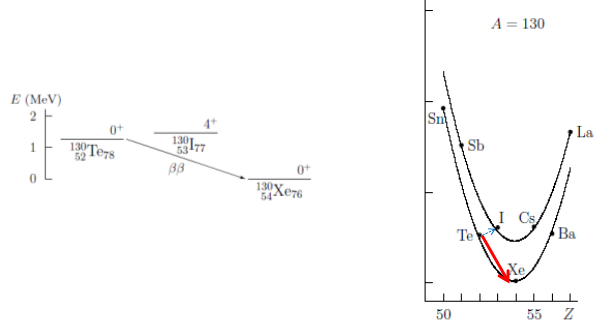
\includegraphics[scale=0.8]{ch1/image11.png}
	\captionof{figure}{ }
	\end{wrapfigure}
où l'on a introduit la \textbf{constante diélectrique}
\begin{equation}
\kappa \left( {r,\omega } \right) = 1 + \tilde \chi \left( {r,\omega } \right) = {(n - j\alpha c/2\omega )^2} \approx {n^2}
\end{equation}
L'atténuation étant négligeable, $\kappa$ sera réel. Le milieu étant homogène dans le
cœur et la gaine
\begin{equation}
\nabla  \times \nabla  \times {\bf{\tilde E}} = \nabla \left( {\nabla  \cdot {\bf{\tilde E}}} \right) - \Delta {\bf{\tilde E}} =  - \Delta {\bf{\tilde E}}
\end{equation}
Notons que $\kappa$ sera différent dans le cœur et dans la gaine. On trouve alors six équations (identiques pour $\tilde{H}$) équations\\

\cadre{\textsc{Equation d'Helmotz}\begin{equation}
\Delta {\bf{\tilde E}} + \kappa \left( \omega  \right)\frac{{{\omega ^2}}}{{{c^2}}}{\bf{\tilde E}} = 0\qquad\qquad\qquad
\Delta \tilde H + \kappa \left( \omega  \right)\frac{{{\omega ^2}}}{{{c^2}}}\tilde H = 0
\end{equation}
où $\kappa_{core}\neq\kappa_{cladding}$ où la constante diélectrique dépend de la fréquence et où
\begin{equation}
{\kappa _j}\left( \omega  \right)\frac{{{\omega ^2}}}{{{c^2}}} = {n_j}^2\left( \omega  \right)\frac{{{\omega ^2}}}{{{c^2}}} = {n_j}^2\left( \omega  \right){\left( {\frac{{2\pi }}{{{\lambda _0}}}} \right)^2} = {n_j}^2\left( \omega  \right)k_0^2
\end{equation}
avec $j=1$ pour le cœur et $j=2$ pour la gaine.}\ \\

Nous avons donc six équations couplées. Heureusement, seulement deux sont indépendantes : il ne 
faudra résoudre que ces deux-là
\begin{equation}
{\tilde E_y} = {\tilde E_y}({\tilde E_x},{\tilde H_x})\qquad\qquad
{\tilde H_y} = {\tilde H_y}({\tilde E_x},{\tilde H_x})\qquad\qquad
{\tilde E_z} = {\tilde E_z}({\tilde E_x},{\tilde H_x})\qquad\qquad
{\tilde H_z} = {\tilde H_z}({\tilde E_x},{\tilde H_x})
\end{equation}

Le schéma de résolution sera alors le suivant
\begin{enumerate}
\item Tenir compte des symétries de la structure en $(x,y,z)$
\item Séparer le problème pour chaque milieu homogène (cœur et gaine)
\item Appliquer les CL aux interfaces cœur-gaine pour trouver les modes guidés.
\begin{itemize}
\item[$\bullet$] Il faut aussi avoir la continuité des composantes tangentielle de $\vec{E}$ et 
$\vec{E}$ ainsi que les composantes normales de $\vec{B}$ et $\vec{D}$.
\end{itemize}
\item Construire la solution générale (équation linéaire)
\end{enumerate}\ 

La solution générale d'un champ EM dans un guide d'onde est la suivante (idem pour $\tilde{H}$)
\begin{equation}
\tilde E(x,y,z,\omega ) = \sum\limits_m {\left[ {{a_m}{{\tilde E}_m}(x,y,z,\omega ) + {a_{ - m}}{{\tilde E}_{ - m}}(x,y,z,\omega )} \right] + {{\tilde E}_{{\rm{rad}}}}(x,y,z,\omega )} 
\end{equation}
où le premier terme sont les modes progressif, la second les régressif et le dernier, le champ 
radiés (négligeable). 

\subsubsection{Étape 1 : Symétries}
Basé sur les symétries, nous allons chercher par la méthode de séparation des variables une solution
de la forme
\begin{equation}
{E_x}(x,y,z,t) = {\tilde E_x}(x,y,z,\omega )\exp (j\omega t) = {E_x}(x).Y(y).Z(z).\exp (j\omega t)
\end{equation}
et de même pour $H_x$. Nous pouvons procéder à une telle résolution par symétrie de translation en $y,
z$ et dans le temps. Si nous avions un guide plan rectangulaire entouré d'une gaine optique, nous
aurions une seule fonction en $z$, une en $t$ mais également une en $x$ et $y$ ! \\

Nous avons donc
\begin{equation}
\frac{1}{{{{\rm{E}}_x}}}\frac{{{d^2}{{\rm{E}}_x}}}{{d{x^2}}} + \frac{{{\omega ^2}}}{{{c^2}}}\kappa (\omega ,x) + \frac{1}{{\rm{Y}}}\frac{{{d^2}Y}}{{d{y^2}}} + \frac{1}{{\rm{Z}}}\frac{{{d^2}Z}}{{d{z^2}}} = 0
\end{equation}
En $Y$ et $Z$, nous pouvons avoir des solutions exponentielles, sinus, cosinus, sinh et cosh. Il faut
comprendre l'invariance en translation en terme de densité de photon. Comme celui-ci contient un 
module carré, il faut choisir la solution en exponentielles imaginaires. Ceci signifie que les 
"constantes" que vaut ces termes doit être négative. On en tire pour $Y$
\begin{equation}
\frac{1}{{\rm{Y}}}\frac{{{d^2}Y}}{{d{y^2}}} =  - {\gamma ^2}\qquad\qquad\Rightarrow\qquad\qquad
{\rm{Y(}}y{\rm{)}} = {e^{ - j\gamma y}}
\end{equation}
où $\gamma\in\mathbb{R}$. Pour $Z$
\begin{equation}
\frac{1}{{\rm{Z}}}\frac{{{d^2}Z}}{{d{z^2}}} =  - {\beta ^2} \qquad\qquad\Rightarrow\qquad\qquad
{\rm{Z(}}z{\rm{)}} = {e^{ - j\beta z}}
\end{equation}
où $\beta\in\mathbb{R}$. L'équation à résoudre devient alors
\begin{equation}
\frac{{{d^2}{{\rm{E}}_x}}}{{d{x^2}}} + \left[ {\frac{{{\omega ^2}}}{{{c^2}}}\kappa (\omega ,x) - {\beta ^2} - {\gamma ^2}} \right]{{\rm{E}}_x} = 0\qquad\qquad
\frac{{{d^2}{{\rm{H}}_x}}}{{d{x^2}}} + \left[ {\frac{{{\omega ^2}}}{{{c^2}}}\kappa (\omega ,x) - {\beta ^2} - {\gamma ^2}} \right]{{\rm{H}}_x} = 0
\end{equation}
Celles-ci possèdent comme solutions
\begin{equation}
{E_x} = {{\rm{E}}_x}(x)\exp (j[\omega t - \beta z - \gamma y])\qquad\qquad
{H_x} = {{\rm{H}}_x}(x)\exp [j(\omega t - \beta z - \gamma y)]
\end{equation}
où $E_x(x)$ et $H_x(x)$ sont à déterminer. Comme $E$ et $H$ ont un module indépendant de $y,z$ et 
$t$, ces solutions sont les \textbf{modes du guide d'onde}.\\

Il existe deux types de solutions pour un guide plan
\begin{description}
\item[Mode TE] Le champ électrique est hors du plan, quelque soit la réflexion et la polarisation. 
De même pour le champ magnétique. On parle de \textit{transverse électrique} car l'énergie se propage
dans la direction $z$ et non $k$ : la projection de $E$ sur $z$ est nulle.
\item[Mode TM] Ici la projection de $E$ sur $z$ est non-nulle. Le champ n'est pas ici perpendiculaire à la direction de propagation. En guidage faible, l'angle est proche de $90^\circ$ et la composante
en $z$ est très petite mais non-nulle.
\end{description}

\begin{center}
	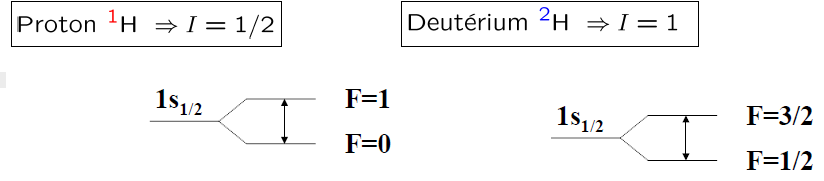
\includegraphics[scale=0.75]{ch1/image12.png}
	\captionof{figure}{ }
\end{center}


Nous allons considérer le mode TE\footnote{Je comprends pas trop pourquoi on fait ça ici.} tel que $E_x=0$. Les équations de Maxwell deviennent (voir Annexes)
\begin{equation}
{E_y} =  - \frac{{\beta {\rm{ }}\omega {\rm{ }}{\mu _0}}}{{{\gamma ^2} + {\beta ^2}}}{\rm{ }}{H_x}\qquad
{E_z} =  - \frac{{\gamma {\rm{ }}\omega {\rm{ }}{\mu _0}}}{{{\gamma ^2} + {\beta ^2}}}{\rm{ }}{H_x}\qquad
{H_y} =  - j\frac{\gamma }{{{\gamma ^2} + {\beta ^2}}}{\rm{ }}\frac{d}{{dx}}{H_x}\qquad
{H_z} =  - j\frac{\beta }{{{\gamma ^2} + {\beta ^2}}}{\rm{ }}\frac{d}{{dx}}{H_x}
\end{equation}
Une onde dans un guide infini est équivalent à une onde plane : pas de profil en $Y$ ou $Z$. On peut
alors définir $Z$ comme la direction dans laquelle se propage ce qui signifie que $\gamma=0$ car 
aucune phase n'est accumulée dans cette direction. Dès lors, $E_x=E_z=0$ (TE) et $H_y=0$)
\begin{equation}
{H_x} =  - \frac{{\beta {\rm{ }}}}{{\omega {\rm{ }}{\mu _0}}}{\rm{ }}{E_y},\qquad\qquad
{H_z} = \frac{{ - j}}{\beta }{\rm{ }}\frac{d}{{dx}}{H_x} = \frac{j}{{\omega {\rm{ }}{\mu _0}}}\frac{d}{{dx}}{E_y}
\end{equation}
où
\begin{equation}
\frac{{{d^2}{{\rm{E}}_y}}}{{d{x^2}}} + \left[ {\frac{{{\omega ^2}}}{{{c^2}}}{\kappa _j}(x) - {\beta ^2}} \right]{{\rm{E}}_y} = 0
\end{equation}
Faisons de même pour $H_x=0$. Nous avons $H_x=H_z=0$ (TM) et $E_y=0$ :
\begin{equation}
{E_x} = \frac{{\beta {\rm{ }}}}{{\omega {\rm{ }}{\varepsilon _0}{\rm{ }}\kappa }}{\rm{ }}{H_y}\qquad\qquad
{E_z} = \frac{{ - j}}{{\omega {\rm{ }}{\varepsilon _0}{\rm{ }}\kappa }}{\rm{ }}\frac{d}{{dx}}{H_y}
\end{equation}
où
\begin{equation}
\frac{{{d^2}{{\rm{H}}_y}}}{{d{x^2}}} + \left[ {\frac{{{\omega ^2}}}{{{c^2}}}{\kappa _j}(x) - {\beta ^2}} \right]{{\rm{H}}_y} = 0
\end{equation}

\cadre{\begin{center}
Un champ EM solution des équations de Maxwell dans un guide plan est une ainsi une \textbf{
combinaison linéaire} des modes TE et TM du guide d'onde.
\end{center}}\ \\


\subsubsection{Étape 2 : Résolution par milieu homogène}
Le guide d'onde est symétrique $\kappa(x)=\kappa(-x)$. L'intensité, proportionnelle au module carré 
$|E|^2$ est aussi symétrique. Les modes doivent alors être pairs ou impairs.\\

Intéressons-nous aux modes TE avec $\gamma=0$
\begin{equation}
\frac{{{d^2}{{\rm{E}}_y}}}{{d{x^2}}} + \left[ {\frac{{{\omega ^2}}}{{{c^2}}}{\kappa _j}(x) - {\beta ^2}} \right]{{\rm{E}}_y} = 0
\end{equation}
et plus particulièrement au cas où $E_y$ est symétrique (fonction paire de $x$). Il faut trouver une
solution symétrique satisfaisant les CL Dans la gaine $(|x|>a)$, nous voulons une atténuation afin d'avoir un maximum d'énergie dans le cœur
\begin{equation}
{{\rm{E}}_y} = {{\rm{A}}_{{\rm{sym}}}}\cos (\sigma a).\exp \left[ { - \xi (x - a)} \right]
\end{equation}
Dans le coeur $(|x|\leq a)$ nous pouvons avoir un cos ou un cosh. La seule solution acceptable est 
$\cos$ car elle respecte la continuité de la dérivée première\footnote{$H_z$ doit être continue et
elle dépend de la dérivée de $E_y$ par rapport à $x$.}
\begin{equation}
{{\rm{E}}_y} = {{\rm{A}}_{{\rm{sym}}}}\cos (\sigma x)
\end{equation}
La seule solution possible est un cos dans le cœur et une exponentielle décroissante dans la gaine. 
La continuité de $E_y$ en $x=a$ est alors vérifiée. 
\begin{center}
	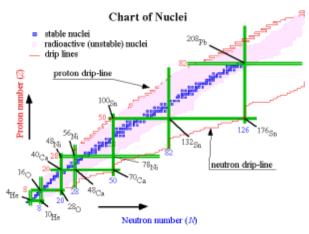
\includegraphics[scale=0.75]{ch1/image13.png}
	\captionof{figure}{ }
\end{center}

Dans les précédentes équations, nous avons posé
\begin{equation}
{\sigma ^2} = \frac{{{\omega ^2}}}{{{c^2}}}{\kappa _1} - {\beta ^2} = k_0^2n_1^2 - {\beta ^2}
\end{equation}
et
\begin{equation}
{\xi ^2} = {\beta ^2} - \frac{{{\omega ^2}}}{{{c^2}}}{\kappa _2} = {\beta ^2} - k_0^2n_2^2
\end{equation}
Quels sont les signes de $\sigma^2$ et $\xi^2$ ? 
\begin{itemize}
\item[$\bullet$] ${\sigma ^2} = k_0^2n_1^2 - {\beta ^2} > 0$ : $\sigma$ doit être réel pour 
satisfaire les CL
\item[$\bullet$] ${\xi ^2} = {\beta ^2} - k_0^2n_2^2 > 0$ : $\xi$ est réel. S'il est positif, on a
bien une décroissance exponentielle dans la gaine
\begin{equation}
\text{Mode quidé}\qquad\Leftrightarrow\qquad \beta > n_2k_0
\end{equation}
\item[$\bullet$] ${\xi ^2} = {\beta ^2} - k_0^2n_2^2 < 0$ : $\xi$ est imaginaire : oscillation 
dans la gaine
\begin{equation}
\text{Mode faible}\qquad\Leftrightarrow\qquad \beta^2> n_2^2k_0^2
\end{equation}
\end{itemize}\

Compte-tenu des conclusions ci-dessus, nousnaurons un mode quidé que si\\

\cadre{\textsc{Mode guidé si }\begin{equation}
n_nk_0>\beta > n_2k_0\qquad\Leftrightarrow\qquad n_1>n_2
\end{equation}}\ \\

Il s'agit bien ici d'un résultat, et non quelque chose que nous avons imposé comme c'était le cas
dans l'optique géométrique.


\subsubsection{Étape 3 : Condition de continuité à l'interface cœur-gaine}
Comme l'indique le nom de la sous-sous-section, il faut garantir la continuité de $H_z$ en 
$x=\pm a$, impliquant la continuité de la dérivée de $E_y$ en ce point. On trouve alors une 
branche de cosinus comme solution dans le cœur ($|x|\leq a$)
\begin{equation}
{H_z} = \frac{j}{{\omega {\rm{ }}{\mu _0}}}\frac{d}{{dx}}{E_y}\qquad\Rightarrow\qquad
{{\rm{H}}_z} =  - \frac{{j\sigma }}{{\omega \;{\mu _0}}}{{\rm{A}}_{{\rm{sym}}}}\sin (\sigma x)
\end{equation}
Et dans la gaine ($|x|>a$, déjà particularisé au point $a$)
\begin{equation}
{{\rm{H}}_z} =  \pm \frac{{ - j\xi }}{{\omega \;{\mu _0}}}{{\rm{A}}_{{\rm{sym}}}}\cos (\sigma a).\exp \left[ { - \xi (x - a)} \right]
\end{equation}
On en tire
\begin{equation}
 \pm \frac{{j\sigma }}{{\omega \;{\mu _0}}}{{\rm{A}}_{{\rm{sym}}}}\sin (\sigma a) =  \pm \frac{{j\xi }}{{\omega \;{\mu _0}}}{{\rm{A}}_{{\rm{sym}}}}\cos (\sigma a)
\end{equation}
D'où
\begin{equation}
\tan (\sigma a) = \frac{{\xi .a}}{{\sigma .a}}
\end{equation}

\begin{wrapfigure}[14]{l}{7.5cm}
	\vspace{-9mm}
	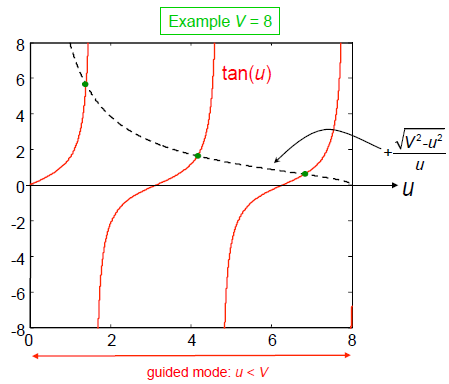
\includegraphics[scale=0.6]{ch1/image14}
	\captionof{figure}{3 solutions TE symétriques ($V=8$)}
	\end{wrapfigure}
Cette relation doit être vérifiée pour garantir la continuité. Toutes les solutions en termes de 
$\sigma$ vont être les solutions correspondant à un mode guidé. En posant les fonctions 
adimensionnelle $u \buildrel \Delta \over = \sigma .a = a.{(k_0^2n_1^2 - {\beta ^2})^{1/2}}$ et ${V^2} \buildrel \Delta \over = {a^2}({\xi ^2} + {\sigma ^2}) = {a^2}k_0^2(n_1^2 - n_2^2)$, on peut définir la \textbf{fréquence normalisée du guide d'onde}
\begin{equation}
V = a{k_0}\sqrt {n_1^2 - n_2^2} 
\end{equation}
où ${V^2} - {u^2} = {V^2} - {a^2}{\sigma ^2} = {a^2}{\xi ^2} > 0$ pour avoir un mode guidé ($\xi^2 > 0$ et $\xi > 0$). Physiquement, seule la valeur 
positive de $\xi$ convient sans quoi il y aurait une croissance infinie dans la gaine\\

\cadre{\begin{equation}
{\rm{tan(}}u{\rm{) =  + }}\frac{{\sqrt {{V^{\rm{2}}}{\rm{ -  }}{u^{\rm{2}}}} }}{u}
\end{equation}
Connaissant $\omega$ et l'index, il n'y a dès lors qu'un nombre \textbf{limité} de valeurs 
de $\sigma$ (et donc de $\beta$) satisfaisant à cette équation. Chaque $\beta$ \textbf{identifie}
un \textbf{mode guidé particulier}.}\ \\

Le même raisonnement peut être fait en partant d'un champ $E_y$ antisymétrique. On trouve alors\ \\

\cadre{\begin{equation}
{\rm{tan(u) =   -  }}\frac{{\rm{u}}}{{\sqrt {{{\rm{V}}^{\rm{2}}}{\rm{ -  }}{{\rm{u}}^{\rm{2}}}} }}
\end{equation}}\ \\

Ce qui est semblable à la précédente relation avec un signe négatif et une inversion 
numérateur/dénominateur\footnote{Voir slides 29-30 pour plus de détails.}. Pour $V=8$, il existe
également trois solutions TE, mais cette fois-ci antisymétriques. Comme la fonction rouge est 
tangente, il y aura toujours au moins un mode guidé. La fibre deviendra multimode dès la première
asymptote de cette fonction, à savoir en $u=\pi/2$.

\newpage
\begin{wrapfigure}[14]{l}{7.2cm}
	\vspace{-2mm}
	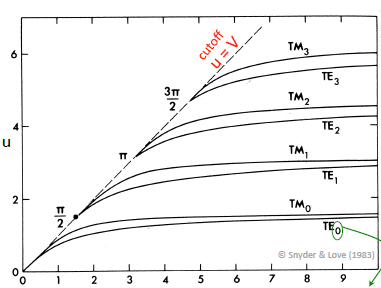
\includegraphics[scale=0.65]{ch1/image15}
	\captionof{figure}{ }
	\end{wrapfigure}
On peut faire le même calcul pour les modes $TM$ avec $\gamma=0 (E_x=E_z=H_y=0$). En évaluant la 
continuité, on retombe sur une équation aux valeurs propres pour les modes $TM$. Les conclusions
sont semblables : il y a toujours au moins un mode $TM$ et la valeur de la fréquence normalisée
à partir de la quelle on en voit d'autres est également $\pi/2$. \\

Le nombre de modes guidés augmente donc avec l'augmentation de la fréquence normalisée $V$. Dès 
lors, le guide est \textbf{monomode} si\\

\cadre{\begin{equation}
V < \dfrac{\pi}{2}
\end{equation}}\ \\

Les observateurs diront qu'il y a deux modes guidés en dessous de cette valeur (léger écart entre
$TE$ et $TM$). C'est vrai, mais on parle toujours de monomode : l'un ou l'autre sera excité en 
fonction de la polarisation. Ce léger écart signifie que le $\beta$ est différent pour les deux modes 
: le guide plan est \textit{biréfringeant}.

\subsubsection{Discussions}
\begin{enumerate}
\item \textit{Interprétation de $\beta$}.\\
Choisissons $z$ comme direction de propagation et $\gamma= 0$
\begin{equation}
{E_y} = {{\rm{E}}_y}\exp [j(\omega t - \beta z - \gamma y)] = {{\rm{E}}_y}\exp [j(\omega t - \beta z)]
\end{equation}
Le mode oscille à $\omega$ et accumule une phase dans la direction $z$ donnée par $\beta$ ($m^{-1}$). 
Il s'agit de la \textbf{constante de propagation} du mode. La variation de $\beta$ par rapport à la 
fréquence $\omega$, $\beta(\omega)$ est la \textbf{relation de dispersion du mode}. \\

Cette constante de propagation est bornée
\begin{equation}
\frac{{2\pi }}{{{\lambda _0}}}{n_2} < \beta  = \frac{{2\pi }}{{{\lambda _0}}}{n_{eff}} < \frac{{2\pi }}{{{\lambda _0}}}{n_1}
\end{equation}
où apparait l'indice effectif du mode, qui se rapporte à une mode tout comme $\beta$ : c'est 
l'indice de réfraction "vu" par le mode. Si un mode est fort dans la gaine, son indice effectif sera
proche de $n_2$ et inversement. En terme de vitesse de phase, le mode se propage à une vitesse entre
celle dans le cœur et celle dans la gaine
\begin{equation}
\frac{c}{{{n_1}}} < \frac{\omega }{\beta } < \frac{c}{{{n_2}}}
\end{equation}
La constante de propagation, via $\beta/\omega$, est alors fortement reliée à l'extension modale sur
le cœur et la gaine.
\newpage
\item \textit{Puissance par unité de longueur d'un mode TE}\footnote{Le guide plan étant infini
dans une direction transverse, il faut bien parler \textit{par unité de longueur}.}.
Celle-ci est donnée par l'intégrale de la composante $z$ du vecteur de Poynting moyennée 
temporellement sur $x$, celui-ci définissant la forme du guide
\begin{equation}
{P_u} = \int\limits_{ - \infty }^{ + \infty } {\left\langle {{S_z}} \right\rangle dx} 
\end{equation}
On en tire $\left\langle {{S_z}} \right\rangle  = \frac{\beta }{{2\;\omega \;{\mu _0}}}\;\;{E_y}{^2}$
et ${P_u} = 2\int\limits_0^{ + \infty } {\frac{\beta }{{2\;\omega \;{\mu _0}}}\;\;{E_y}{^2}dx}$. 
Pour les modes TE symétriques, en décomposant entre le cœur (première intégrale) et la gaine (la
seconde)
\begin{equation}
{P_u} = \frac{\beta }{{\omega \;{\mu _0}}}\left[ {\int\limits_0^a {\;{{({{\rm{A}}_{{\rm{sym}}}}\cos (\sigma x))}^2}dx + \int\limits_a^{ + \infty } {\;{{({{\rm{A}}_{{\rm{sym}}}}\cos (\sigma a).\exp \left[ { - \xi (x - a)} \right])}^2}dx} } } \right]
\end{equation}
On en tire
\begin{equation}
{P_u} = \frac{\beta }{{2\;\omega \;{\mu _0}}}{\rm{A}}_{{\rm{sym}}}^2[a + \frac{1}{\xi }]
\end{equation}
où ${h_{{\rm{eff}}}} \buildrel \Delta \over = {\rm{2(}}a{\rm{ + }}\frac{{\rm{1}}}{\xi }{\rm{)}}$ est
l'\textbf{épaisseur effective}. Tout se passe comme si l'énergie se réparti sur cette hauteur. Le
$1/\xi$ traduit bien l'étalement du mode sur la gaine optique, celui-ci n'étant pas bloqué dans le
cœur.
\item \textit{Profil transverse}\\
Considérons le cas précédemment abordé d'un mode $TE$ symétrique où $V=8$. La parité de l'indice 
donne une information sur la parité du mode, mais l'indice donne surtout le nombre de passage
par un zéro au sein du guide. Plus l'ordre du mode augmente, plus la complexité (nombre de nœud) du
mode fait de même. 

\begin{center}
	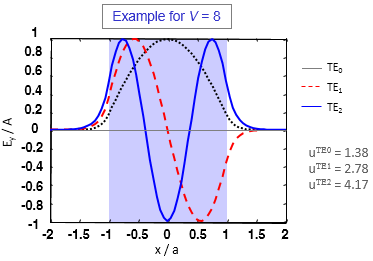
\includegraphics[scale=0.75]{ch1/image16.png}
	\captionof{figure}{ }
\end{center}

Notons que la partie évanescente du mode augmente avec l'ordre du mode lorsque $x$ diminue (l'indice
effectif se rapproche ainsi de $n_2$) : $\beta$ diminue avec l'ordre du mode.\\

Pour résumer, un grand $V$ implique un grand nombre de mode rimant avec une complexité d'onde guidée.
Il va y avoir superposition des modes guidés. Lorsqu'on excite plus d'un mode (TE/TM), l'intensité
devient dépendant de $z$ car $\beta^N$ diffère pour chaque ordre $N$. La simulation du \textit{slide 
35} met en évidence qu'un champ au début localisé se met à remplir tout le guide. Un champ évanescent
est en pratique toujours présent.\\

Intéressons-nous au profil transverse d'un mode \textit{près de la coupure}, par exemple en $V=1$. 
Plus on se rapproche de la coupure $(u=V$), plus $\xi$ est petit et plus l'extension du mode dans 
la gaine optique est importante (le profil modal étant proportionnel à $e^{-\xi}$, l'extention dans la
gaine augmente drastiquement). Ici, nous sommes
entre la coupure du mode 1 et 2. Par le calcul simple ${h_{{\rm{eff}}}}/(2a{\rm{)}} = {\rm{(1 + }}
\frac{{\rm{1}}}{{\xi .a}}{\rm{)  =  2}}{\rm{.47}}$, 
on voit que le mode est deux fois plus étendu dans le gaine que dans le cœur!
\begin{center}
	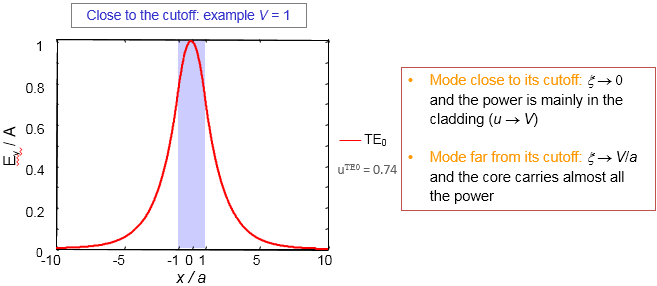
\includegraphics[scale=0.75]{ch1/image17.png}
	\captionof{figure}{ }
\end{center}
Nous sommes donc bien loin des considérations de l'optique géométrique. 

\item \textit{Interprétation du profil modal dans le cœur comme une superposition d'ondes planes}\\
Soit un mode TE symétrique d'ordre $N$
\begin{equation}
E_y^N = {{\rm{A}}_{{\rm{sym}}}}\cos ({u^N}.x/a).{e^{j(\omega t - {\beta ^N}z)}}
\end{equation}
Écrivons-le cosinus comme deux exponentielles 
\begin{equation}
E_y^N = \frac{1}{2}{{\rm{A}}_{{\rm{sym}}}}[{e^{j(\omega t - {\beta ^N}z + {u^N}.x/a)}} + {e^{j(\omega t - {\beta ^N}z - {u^N}.x/a)}}]
\end{equation}
On y voit deux ondes planes
\begin{equation}
{e^{j(\omega t - {\beta ^N}z - {u^N}.x/a)}} = {e^{j(\omega t - {k^N}.r)}}
\end{equation}
où $k_x^N = u^N/a, k_y^N=0$ et $k_z^N=\beta^N$. Calculons alors le module du nombre d'onde
\begin{equation}
\;k\;{^2} = {({u^N}/a)^2} + {({\beta ^N})^2} = {k_0}^2{n_1}^2 = {k_1}^2
\end{equation}
Celui-ci vaut $k_1^2$, soit exactement le nombre d'onde dans un milieu d'indice $n_1$ : il s'agit
d'une onde plane qui se propage.  La constante de propagation $\beta$ n'est que la projection de 
$\vec k_1$ sur la direction de propagation. 

\begin{center}
	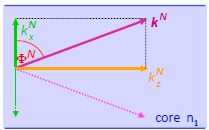
\includegraphics[scale=0.75]{ch1/image18.png}
	\captionof{figure}{ }
\end{center}

Le profil est le résultat des interférences entre
deux ondes planes de vecteur d'onde $(\pm k_x^N,0,\beta^N)$. On peut associer un "rayon" à une
onde plane (direction orthogonale au front d'onde, soit la direction de $k^N$) et retrouver la 
conclusion de l'optique géométrique 
\begin{equation}
\cos ({\Phi ^N}) = \frac{{{u^N}}}{{{k_1}.a}} < \frac{V}{{{k_1}.a}} = \frac{{a.{k_0}}}{{a.{k_0}.{n_1}}}\sqrt {{n_1}^2 - {n_2}^2}  = \sqrt {1 - {n_2}^2/{n_1}^2}  = \cos ({\Phi _c})\Rightarrow
\phi^N > \phi_c
\end{equation}

\item \textit{Ordre de grandeur}. Cf. \textit{slide 38}
\item \textit{Guide plan non symétrique}\\
Considérons $n_3$ comme étant de l'air : peu d'onde évanescante de ce côté, mais beaucoup de l'autre :
le mode est poussé du côté du saut d'indice le plus faible.
\begin{center}
	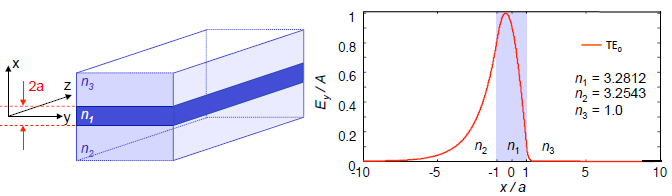
\includegraphics[scale=0.75]{ch1/image19.png}
	\captionof{figure}{ }
\end{center}
 Les solutions trouvées sont cependant
du même type.
\item \textit{Saut d'indice homogène dans un guide rectangulaire}. Pas de calcul analytique possible,
cf. \textit{slide 40}.
\end{enumerate}

\subsection{Guides à saut d'index cylindriques}
	\begin{wrapfigure}[9]{l}{6cm}
	\vspace{-5mm}
	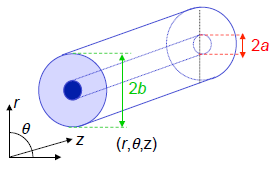
\includegraphics[scale=0.75]{ch1/image20.png}
	\captionof{figure}{ }
	\end{wrapfigure}
L'idée est la même, seule la géométrie va un petit peu compliquer les calculs ! La différence 
principale est que la structure a maintenant deux dimensions transverses : la propagation sera
caractérisée par deux paramètres. Faisons comme 
hypothèses
\begin{itemize}
\item[$\bullet$] Milieu diélectrique, non-magnétique, linéaire, isotropique et sans pertes
\item[$\bullet$] Milieu homogène (guide à saut d'indice, pas à gradient)
\item[$\bullet$] Gaine d'extension infinie ($2b\gg 2a$)
\end{itemize}
Encore une fois, il n'y a \textbf{pas} d'hypothèse sur la taille du cœur. \\

Nous avons dans le cœur ($r\leq a$)
\begin{equation}
\Delta {\bf{\tilde E}} + \kappa \left( \omega  \right)\frac{{{\omega ^2}}}{{{c^2}}}{\bf{\tilde E}} = 0,\qquad\qquad
\kappa \left( \omega  \right) = {n_1}^2\left( \omega  \right)
\end{equation}
Et dans la gaine ($r\geq a$)
\begin{equation}
\Delta \tilde H + \kappa \left( \omega  \right)\frac{{{\omega ^2}}}{{{c^2}}}\tilde H = 0,\qquad\qquad
\kappa \left( \omega  \right) = {n^2}_2\left( \omega  \right)
\end{equation}
Nous allons procéder à une résolution en considérant $E_z\neq 0$ et/ou $H_z\neq 0$ (voir 
\textit{Annexe 1}).

\subsubsection{Étape 1 : Propriété de symétrie, résolution par la méthode de séparation des variables}
La solution est une onde se propageant dans la direction $z$ où $\beta$ - la constante de 
propagation - joue le même rôle que précédemment.
\begin{equation}
\begin{array}{cc}
{E_z} = {\tilde E_z}(x,y)\exp (j[\omega t - \beta z]) & {H_z} = {\tilde H_z}(x,y)\exp (j[\omega t - \beta z])\\
\Downarrow & \Downarrow\\
\frac{{{\partial ^2}{{\tilde E}_z}}}{{\partial {x^2}}} + \frac{{{\partial ^2}{{\tilde E}_z}}}{{\partial {y^2}}} + [\kappa (\omega )\frac{{{\omega ^2}}}{{{c^2}}} - {\beta ^2}]{\tilde E_z} = 0
 & \frac{{{\partial ^2}{{\tilde H}_z}}}{{\partial {x^2}}} + \frac{{{\partial ^2}{{\tilde H}_z}}}{{\partial {y^2}}} + [\kappa (\omega )\frac{{{\omega ^2}}}{{{c^2}}} - {\beta ^2}]{\tilde H_z} = 0
\end{array}
\end{equation}
Vu la symétrie du problèmes, nous allons le traiter en symétrie cylindrique
\begin{equation}
x = r\cos (\theta ),\quad
y = r\sin (\theta ),\quad
r = \sqrt {{x^2} + {y^2}},\quad
\theta  = \arctan (\frac{y}{x})
\end{equation}
Dès lors, on trouve  $\frac{\partial }{{\partial x}} = \frac{x}{r}\frac{\partial }{{\partial r}} - \frac{y}{{{r^2}}}\frac{\partial }{{\partial \theta }}$ et $\frac{\partial }{{\partial y}} = \frac{y}{r}\frac{\partial }{{\partial r}} + \frac{x}{{{r^2}}}\frac{\partial }{{\partial \theta }}$. Nos 
champs s'écrivent
\begin{equation}
{\tilde E_r} = {\tilde E_x}\cos (\theta ) + {\tilde E_y}\sin (\theta ),\qquad\qquad
{\tilde E_\theta } =  - {\tilde E_x}sin(\theta ) + {\tilde E_y}\cos (\theta )
\end{equation}
En utilisant les nouvelles composantes de $\vec{E}$ et le Laplacien en coordonnées cylindriques, on 
trouve
\begin{equation}
\frac{{{\partial ^2}{{\tilde E}_z}}}{{\partial {r^2}}} + \frac{1}{r}\frac{{\partial {{\tilde E}_z}}}{{\partial r}} + \frac{1}{{{r^2}}}\frac{{{\partial ^2}{{\tilde E}_z}}}{{\partial {\theta ^2}}} + [\kappa (\omega )\frac{{{\omega ^2}}}{{{c^2}}} - {\beta ^2}]{\tilde E_z} = 0
\end{equation}
Et de même pour $H_z$. Actuellement, $\beta$ n'est pas connue. Nous allons chercher les solutions
physiquement acceptables et chercher à ce qu'elles satisfont les CL. Ceci fixera les valeurs de 
$\beta$ acceptable : elles formeront un ensemble discret, une valeur par mode.\\

Le problème à résoudre est donc
\begin{equation}
\left\{\begin{array}{l}
\DS \frac{{{\partial ^2}{{\tilde E}_z}}}{{\partial {r^2}}} + \frac{1}{r}\frac{{\partial {{\tilde E}_z}}}{{\partial r}} + \frac{1}{{{r^2}}}\frac{{{\partial ^2}{{\tilde E}_z}}}{{\partial {\theta ^2}}} + [\kappa (\omega )\frac{{{\omega ^2}}}{{{c^2}}} - {\beta ^2}]{\tilde E_z} = 0\vspace{2mm}\\
\DS\frac{{{\partial ^2}{{\tilde H}_z}}}{{\partial {r^2}}} + \frac{1}{r}\frac{{\partial {{\tilde H}_z}}}{{\partial r}} + \frac{1}{{{r^2}}}\frac{{{\partial ^2}{{\tilde H}_z}}}{{\partial {\theta ^2}}} + [\kappa (\omega )\frac{{{\omega ^2}}}{{{c^2}}} - {\beta ^2}]{\tilde H_z} = 0\DS\vspace{2mm}\\
\DS{\tilde E_r} =  - \frac{j}{{\kappa {\omega ^2}/{c^2} - {\beta ^2}}}\left( {\beta \frac{{\partial {{\tilde E}_z}}}{{\partial r}} + {\mu _0}\omega \frac{1}{r}\frac{{\partial {{\tilde H}_z}}}{{\partial \theta }}} \right)\DS\vspace{2mm}\\
\DS{\tilde E_\theta } =  - \frac{j}{{\kappa {\omega ^2}/{c^2} - {\beta ^2}}}\left( {\beta \frac{1}{r}\frac{{\partial {{\tilde E}_z}}}{{\partial \theta }} - {\mu _0}\omega \frac{{\partial {{\tilde H}_z}}}{{\partial r}}} \right)\DS\vspace{2mm}\\
\DS{\tilde H_\theta } =  - \frac{j}{{\kappa {\omega ^2}/{c^2} - {\beta ^2}}}\left( {\beta \frac{1}{r}\frac{{\partial {{\tilde H}_z}}}{{\partial \theta }} + \omega \;\varepsilon (\omega )\frac{{\partial {{\tilde E}_z}}}{{\partial r}}} \right)\DS\vspace{2mm}\\
\DS{\tilde H_r} =  - \frac{j}{{\kappa {\omega ^2}/{c^2} - {\beta ^2}}}\left( {\beta \frac{{\partial {{\tilde H}_z}}}{{\partial r}} - \omega \;\varepsilon (\omega )\frac{1}{r}\frac{{\partial {{\tilde E}_z}}}{{\partial \theta }}} \right)\DS
\end{array}\right.
\end{equation}
Auquel il faut joindre $\kappa(\omega)$ du cœur et de la gaine ainsi que les conditions de continuité
en $r=a$ de aux limites périodiques de $2\pi$ en $\theta$. On peut déjà souligner que $E_r$ dépend
de la dérivée de $E_z$ par rapport à $r$ et de $H_z$ par rapport à $\theta$ : les dérivées sont 
"mélangées" (cela aura de l'importance pour les CL).\\

Nous allons séparer la dépendance des solutions en $r$ et $\theta$ : ${\tilde E_z} = {R_z}(r)\;{\Theta
_z}(\theta )$, ce qui se justifie par la symétrie de rotation de la structure. On en tire
\begin{equation}
\frac{{{\partial ^2}{\Theta _z}}}{{\partial {\theta ^2}}} + {N^2}{\Theta _z} = 0,\qquad
\frac{{{\partial ^2}{R_z}}}{{\partial {r^2}}} + \frac{1}{r}\frac{{\partial {R_z}}}{{\partial r}} + [\kappa (\omega )\frac{{{\omega ^2}}}{{{c^2}}} - {\beta ^2} - \frac{{{N^2}}}{{{r^2}}}].\;{R_z} = 0
\end{equation}
où $N^2$ est positif pour avoir un terme oscillant, mais également la périodicité (celui-ci va 
définir la période du terme oscillant). Les fonction $\Theta_z$ et $R_z$ sont pour le moment 
inconnues.

\subsubsection{Étape 2 : Résolution du problème dans le cœur et la gaine optique}
La solution de l'équation azimutale (dépendance angulaire du champ) en $\Theta_z$ est une 
fonction harmonique à cause de la périodicité de $2\pi$ de la structure
\begin{equation}
\frac{{{\partial ^2}{\Theta _z}}}{{\partial {\theta ^2}}} + {N^2}{\Theta _z} = 0
\end{equation}
Dès lors, $N$ est forcément entier : c'est le nombre angulaire du mode
\begin{equation}
\;{\Theta _z}(\theta ) = \left\{ {\begin{array}{*{20}{c}}
{\cos (N\theta )}\\
{\sin (N\theta )}
\end{array}} \right.\qquad N= 0, \pm 1, \pm 2, \dots
\end{equation}
La seconde équation différentielle (partie radiale)
\begin{equation}
\frac{{{\partial ^2}{R_z}}}{{\partial {r^2}}} + \frac{1}{r}\frac{{\partial {R_z}}}{{\partial r}} + [\kappa (\omega )\frac{{{\omega ^2}}}{{{c^2}}} - {\beta ^2} - \frac{{{N^2}}}{{{r^2}}}].\;{R_z} = 0
\end{equation}
Peut s'écrire
\begin{itemize}
\item[$\bullet$] Si $\kappa\omega^2/c^2 - \beta^2 > 0$
\begin{equation}
{{\rm{x}}^2}\frac{{{d^2}{G_N}}}{{d{x^2}}} + x\frac{{d{G_N}}}{{dx}} + ({x^2} - {N^2}){G_N} = 0
\end{equation}
Si $N$ est entier, la dépendance radiale est une \textit{fonction de Bessel}
\item[$\bullet$] Si $\kappa\omega^2/c^2 - \beta^2 > 0$
\begin{equation}
{{\rm{x}}^2}\frac{{{d^2}{G_N}}}{{d{x^2}}} + x\frac{{d{G_N}}}{{dx}} - ({x^2} + {N^2}){G_N} = 0
\end{equation}
Si $N$ est entier, la dépendance radiale est une \textit{fonction de Bessel modifiée}
\end{itemize}
Notons que les deux conditions énoncées ici sont semblables à celle trouvée pour le guide plan.

\begin{center}
	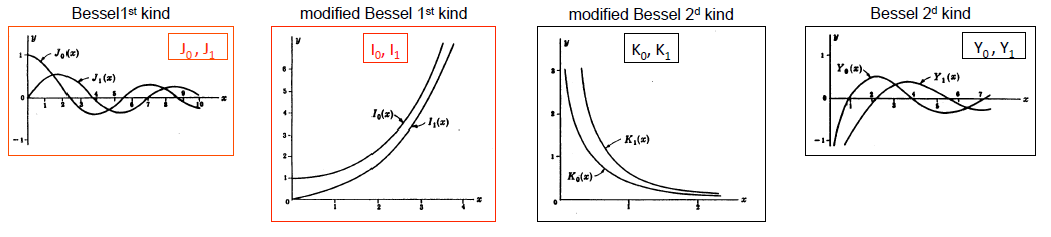
\includegraphics[scale=0.6]{ch1/image21.png}
	\captionof{figure}{La deuxième espèce diverge en 0. Dans le cœur, $J_k$ est acceptable mais pas 
$I_k$ à cause de la divergence. $I_k$ est également acceptable. Dans la gaine, $J_k$ 
n'est pas acceptable car la décroissance de l'amplitude est trop faible, mais $K_k$ est 
bon. Lesquelles prendre ? Nous avions vu que les dérivées étaient "mélangées". Comme 
$I_k$ donnerait un point anguleux, cette solution n'est pas acceptable. Nous avons 
finalement $J_k$ dans le cœur et $K_k$ dans la gaine.}
\end{center}

Pour $N$ fixé, un mode guidé est défini par\\

\cadre{\begin{equation}
\left\{\begin{array}{lll}
{R_z}(r) &= A{\vec{J}_N}(\sigma \;r)&\qquad \text{coeur } (x<a)\\
{R_z}(r) &= C{\vec{K}_N}(\xi \;r)&\qquad \text{gaine } (x\geq a)
\end{array}\right.
\end{equation}
Il s'agit de la \textbf{seule} solution possible (champ évanescent dans la gaine, pas de singularité,
champs continus en $x=a$).}\ \\

Pour avoir une solution dans le cœur, il faut que $\sigma^2>0 \Rightarrow n_1k_0>\beta$. Pour que
$K_n$ soit solution dans la gaine optique, il faut que $\xi^2>0 \Rightarrow \beta > n_2k_0$. Le 
mode ne sera guidé que si \\

\cadre{\begin{equation}
\frac{{2\pi }}{\lambda }{n_2} < \beta  < \frac{{2\pi }}{\lambda }{n_1}
\end{equation}
Soit encore $n_2<n_1$.}\ \\

Comme pour les guides d'ondes plan, la vitesse de phase $\omega/\beta$ dépend de 
l'extension sur le cœur \textbf{et} la gaine. Les solutions sont données aux \textit{slides 47} et \textit{48}.

\subsubsection{Classification des modes du nombre azimutal $N$}
\begin{enumerate}
\item Si $N=0$, il n'y a pas de dépendance angulaire. La situation est celle d'un guide plan et on retrouve les modes TE et TM formés par les rayons méridionaux.
\item Si $N\neq 0$, on ne retrouve pas de modes TE ou TM à causes des rayons obliques mais des \textbf{modes hybrides} $EH_{Nq}$ et $HE_{Nq}$. En fixant $N$, on trouvera alors $q$ solutions : se complique à cause des deux indices.
\end{enumerate}

\subsubsection{Étape 3 : Condition de continuité à l'interface cœur-gaine}
Il faut donc trouver pour un nombre azimutal $N$ donné, les $q$ solutions (nombre radial) possibles (s'il y en a). Le système est donné au \textit{slide 50}, mais "seulement" quatre équations sont indépendantes. Le système possède une solution non triviale ssi le déterminant du système est nul. A l'aide d'une insomnie, de l'hypothèse du \textbf{guidage faible} et de l'annexe 3, on trouve\\

\cadre{
\begin{equation}
\dfrac{\vec{J}_{m-1}(u)}{\vec{J}_{m}(u)}=-w\dfrac{\vec{K}_{m-1}(w)}{\vec{K}_{m}(w)}
\end{equation}
où
$$m=\left\{\begin{array}{ll}
1&\qquad\text{Pour les modes $TE_{0q}$ et $TM_{0q}$}\quad (N=0)
\end{array}\right.$$
}







